\documentclass[aspectratio=169,usepdftitle=true]{beamer}

\usepackage[T1]{fontenc}
\usepackage[utf8]{inputenc}
\usepackage{microtype}
\usepackage[english]{babel}
\usepackage{lipsum}
\usepackage{multirow}
\usepackage{amsmath}
\usetheme{dividing-lines}
\usepackage{amsfonts}

\title{Impact of Covid-19 pandemic in health services usage}
%\subtitle{This is madness}
%\institute{Jornada Susie Bayarri 2022}
\license{\ccbysa}

\date{17 June 2022}

\author{Amanda Fern\'andez-Fontelo, Pedro Puig, Montserrat Guill\'en and David Mori\~na}
\email{dmorina@ub.edu}

\outro{Thank you!}
\titleimage{\tikz\node[opacity=.45]{
\includegraphics[width=4cm,height=\height,keepaspectratio]{BUlogo_cmyk-eps-converted-to.pdf}};}

% just an example command
\newcommand\twosplit[3][t]{%
\begin{columns}[#1]
\begin{column}{0.475\linewidth}#2\end{column}\hfill
\begin{column}{0.475\linewidth}#3\end{column}
\end{columns}}

\usepackage[backend=bibtex8,style=alphabetic]{biblatex}
%\addbibresource{example.bib}
\begin{document}

\section{Introduction}
\begin{frame}{Motivation}
\begin{itemize}
 \item There is an enormous global concern around 2019-novel coronavirus (SARS-CoV-2)
infection in the last months, leading the World Health Organization (WHO) to declare
public health emergency in early 2020
 \item The consequences derived from the pandemic
caused by this virus have had a profound effect on many areas of human activity
 \item In addition to the direct consequences, in 2020 a decrease in use of health services has been detected, both those
belonging to the Public Health System and services associated with private health
insurances
\end{itemize}
%    \begin{definition}[Algorithmus]
%        Ein \emph{Algorithmus} ist eine \emph{eindeutige Handlungsvorschrift} zur Lösung eines Problems.
%    \end{definition}
%    \begin{itemize}
%        \item Es existieren verschiedene Darstellungsformen: \begin{itemize}
%            \item Textuell (1. Tue dies, 2. Tue das, 3. Falls \(X\)\ldots)
%            \item Grafisch (Instruktionsabläufe, Graphen, Grafiken, \ldots)
%            \item Pseudocode
%        \end{itemize}
%        \item Klassische Alltagsbeispiele: (Koch-)Rezepte, Gebrauchsanleitungen, \ldots
%    \end{itemize}
\end{frame}

\begin{frame}{Motivation}
\begin{itemize}
 \item The question is to know if, either due to the effect of
postponing visits or due to the consequences of having suffered the virus (persistent Covid
or secondary effects), there will be an excess of claims in 2022 and the following years
 \item There is already evidence of a higher frequency of use of Health services in the Public
System but it is difficult to determine if the highest frequency of
claims that will be observed will be equal to or greater than the infra-loss rate that was
observed during the pandemic period
\end{itemize}
\end{frame}

\section{Proposed model}
\begin{frame}{INAR models}
Let $X_n$ be a process defined by
\begin{equation}
X_n = \alpha_1 \circ X_{n-1} + \ldots + \alpha_k \circ X_{n-k} + W_n,
\end{equation}
where $0 < \alpha_1 < \ldots < \alpha_k$ and $W_n$ is assumed to follow a Poisson
distribution with a fixed mean $\lambda$. 

$X_n$ and $W_n$ are assumed to be independent at any time $n$.
\end{frame}

\begin{frame}{INAR models}
The $\circ$ operator, called \textit{binomial thinning}, is defined as follows:
\begin{equation}
p_j \circ X_{n-j} = \sum_{i=1}^{X_{n-j}} Y_i,
\end{equation}
where $Y_i$ are independent and identically distributed Bernoulli random variables with a probability of
success equal to $p_j$. 

Therefore, if $X_{n-j}=x_{n-j}$, then $p_j \circ X_{n-j}$ is binomially distributed, with number of successes equal to $x_{n-j}$.
\end{frame}

\begin{frame}{Visual model}
\begin{center}
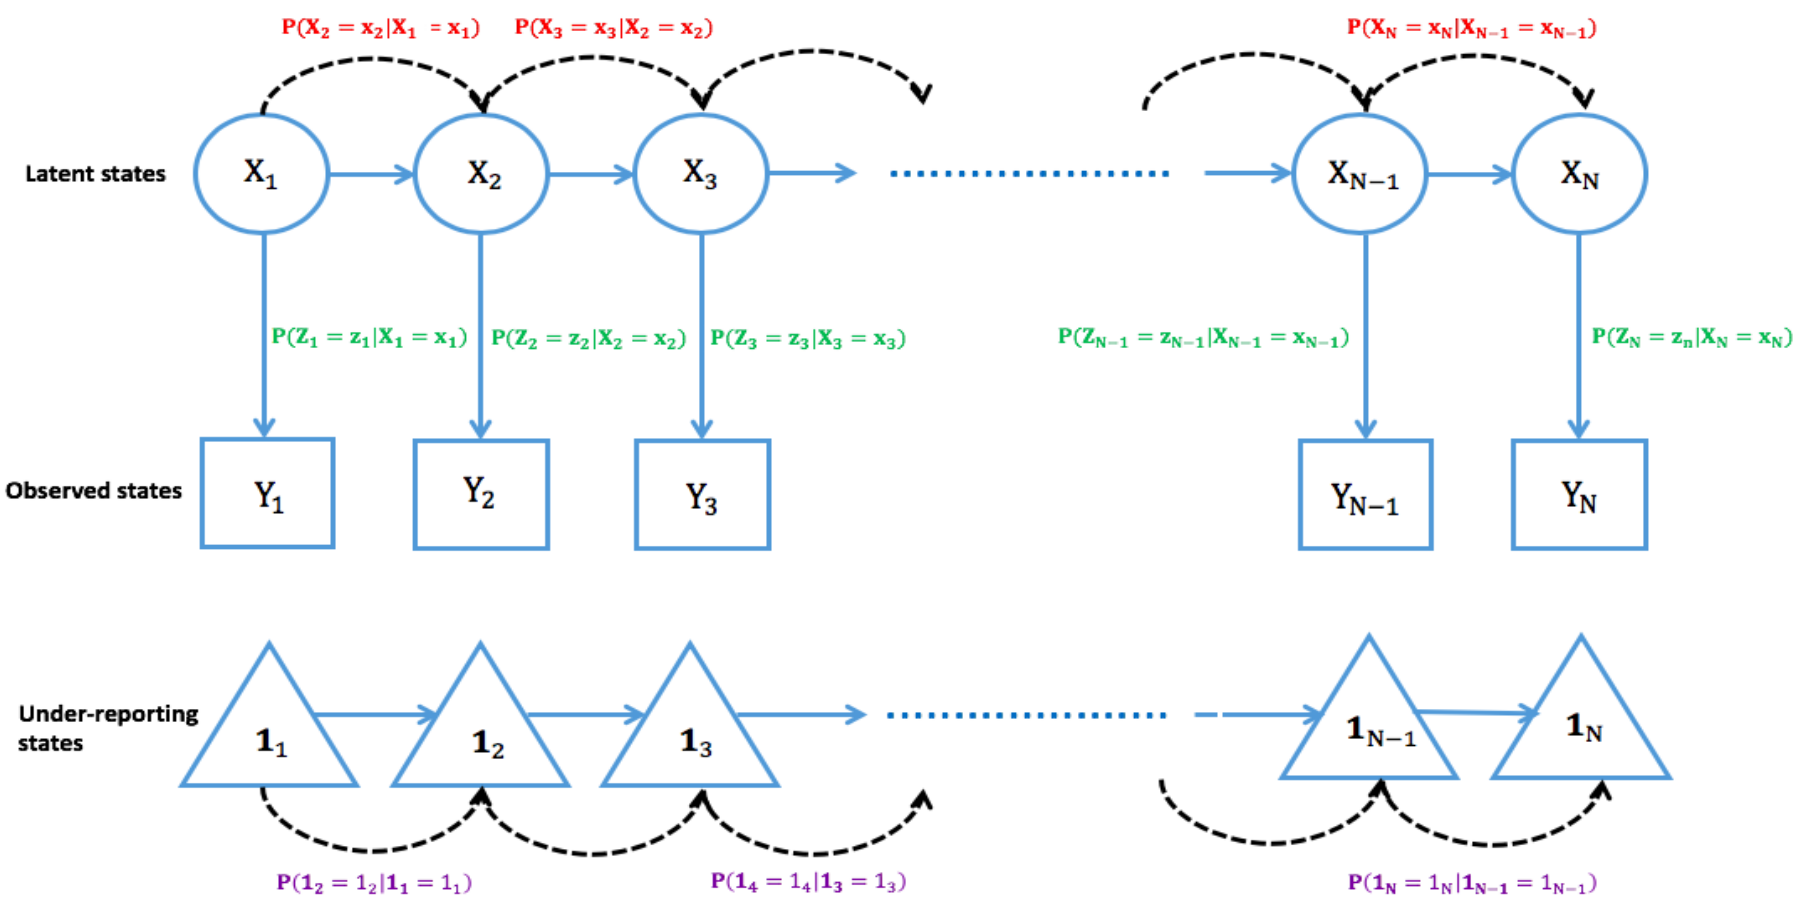
\includegraphics[height=6cm,width=11cm]{HMC.png}
\end{center}
\end{frame}

\begin{frame}[c]{Previously proposed models}
    \begin{block}{Independent under-reporting states}
        \begin{center}
           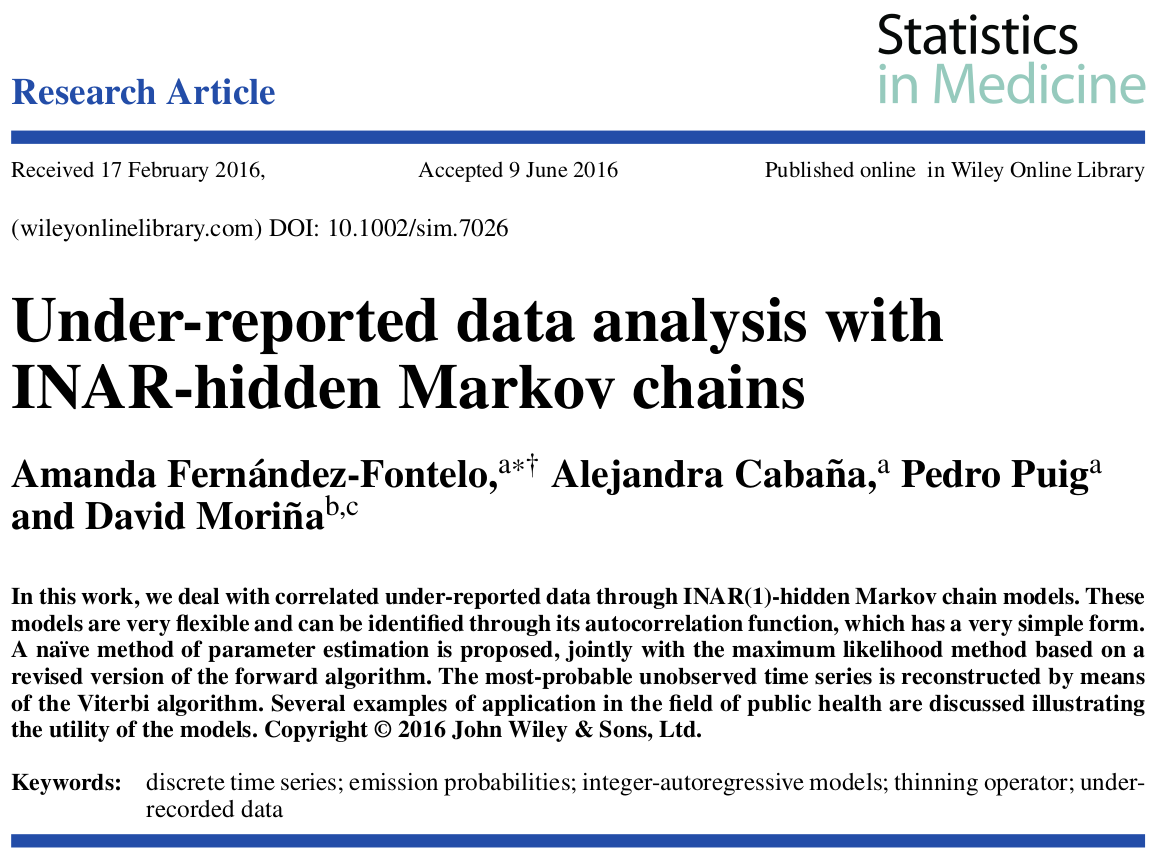
\includegraphics[height=4.7cm,width=7.5cm]{SiM1.png}
        \end{center}
    \end{block}
\end{frame}

\begin{frame}[c]{Previously proposed models}
    \begin{block}{Serially dependent under-reporting states}
        \begin{center}
           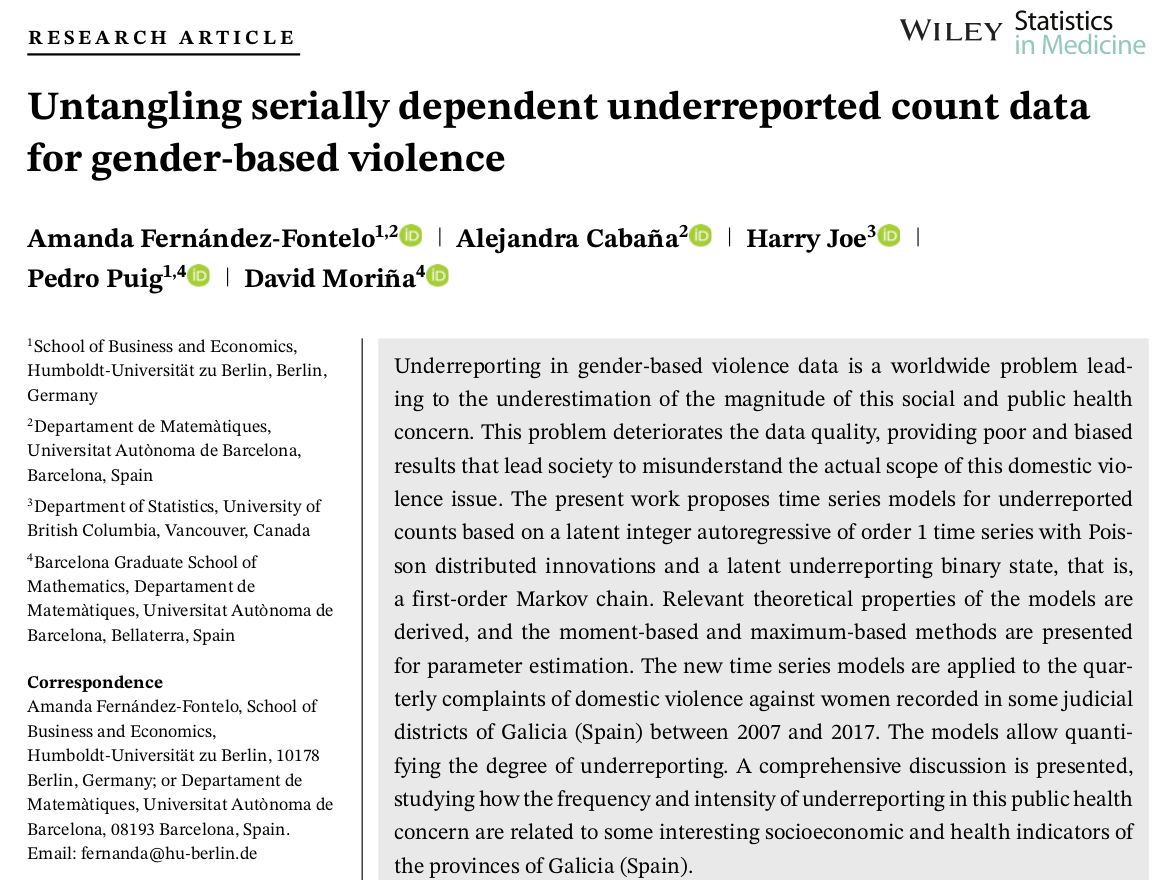
\includegraphics[height=4.7cm,width=7.5cm]{SiM2.png}
        \end{center}
    \end{block}
\end{frame}

\begin{frame}[c]{Previously proposed models}
    \begin{block}{Non-stationary processes}
        \begin{center}
           
\includegraphics[height=4.7cm,width=7.5cm]{Plos.png}
        \end{center}
    \end{block}
\end{frame}

\begin{frame}{The fattening-thinning operator}
Let $X_n$ be a latent process following an INAR(1) structure such that: $X_n=\alpha\circ X_{n-1}+Z_n$, where $\textrm{E}(X_n)=\mu_X$ and $\textrm{Var}(X_n)=\sigma_X^2$ are the expectation and variance of $X_n$, respectively. Assume, for now, that $Z_n \sim \textrm{Poisson}(\lambda)$. Let $Y_n$ be an observed and potentially over- or under-reporting process such that: 
\begin{align}\label{eq0:modelfatthin}
 Y_n=\begin{cases} 
X_n &  1-\omega \\
\theta \Diamond X_n & \omega, \\
   \end{cases}
\end{align}
\end{frame}

\begin{frame}{The fattening-thinning operator}
\noindent $\Diamond$ is the fattening-thinning operator in the sense that:
\begin{align}\label{eq1:fatteringthinning}
\theta \Diamond X_n|X_n=x_n=\sum_{j=1}^{x_n}W_j,
\end{align}

\noindent where $W_j$ are i.i.d random variables defined by the following probability mass function (pmf):

\begin{align}\label{eq2:pmfW}
\mathbb{P}(W_j=k|\phi_1,\phi_2)=\begin{cases} 
1-\phi_1-\phi_2 & \textrm{if } k=0  \\
\phi_1 & \textrm{if } k=1  \\
\phi_2 & \textrm{if } k=2  \\
0 & \textrm{otherwise}, \\
\end{cases}
\end{align}

\noindent where $\theta=(\phi_1,\phi_2)$
\end{frame}

\begin{frame}{Misreported data}
\begin{itemize}
 \item To distinguish between under-reporting, no misreporting or over-
reporting, the following can easily be computed once the model
is estimated:
\end{itemize}
\begin{block}{Under-reporting vs over-reporting}
\begin{table}
\begin{tabular}[h]{cc}
under-reporting: & $\phi_1 + 2 \phi_2 < 1$ \\
no misreporting: & $\phi_1 + 2 \phi_2 = 1$ \\
over-reporting: & $\phi_1 + 2 \phi_2 > 1$
\end{tabular}
\end{table}
\end{block}
\begin{itemize}
 \item Notice that when $\phi_2 = 0$, the model results in simpler versions only accounting for under-reporting or no misreporting.
\end{itemize}
\end{frame}

\subsection{Parameter estimation}
\begin{frame}{Method of moments}
The marginal distribution of the observed process $Y_n$ is
essential to compute the moment-based estimates of the model:
\begin{align}\label{model}
Y_n=\begin{cases} 
\textrm{Poisson}(\mu_X) &  1- \omega \\
\textrm{2nd-order Hermite}(\mu_X \phi_2, \mu_X (1-\phi_1-\phi_2)) & \omega \\
\end{cases}
\end{align}
\begin{enumerate}
 \item Fit the mixture above to obtain estimates of $\omega$, $\mu_X$, $\phi_1$ and $\phi_2$
 \item Use the theoretical expression of the ACF ($\rho_Y$) to estimate $\alpha$
 \item Using $\hat{\mu_X}$ (step 1) and $\hat{\alpha}$ (step 2), $\lambda$ can be easily estimated
\end{enumerate}
\end{frame}

\begin{frame}{Maximum likelihood}
Since the likelihood functions of the processes $Y_n$ and $Z_n$ are directly
intractable (HMC with an infinite number of states), the forward
algorithm is a reasonable choice to compute such functions.
The likelihood is then computed by $P(Y_{1:N}=y_{1:N})=\sum_{x_N=\frac{y_N}{2}, 1_N}^{\infty} \gamma_N (y_{1:N}, x_N, 1_N)$,
where:
\begin{center}
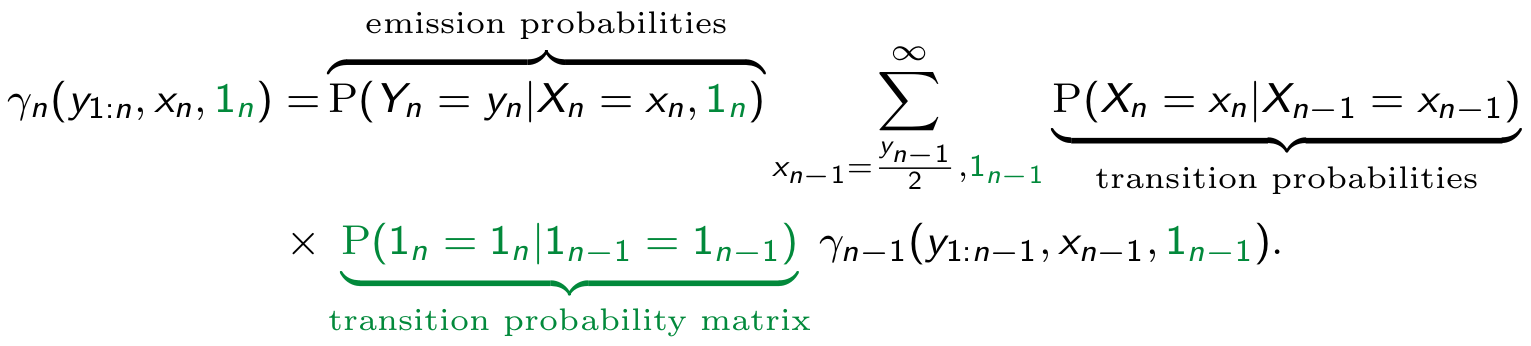
\includegraphics[height=3cm,width=12cm]{gamma_n.png}
\end{center}
\end{frame}

\begin{frame}{Forward probabilities}
\begin{itemize}
 \item While the transition probabilities are easily computed through
the Poisson($\lambda$)-INAR(1) cpmf, the emission probabilities are
trickier:
\end{itemize}
\begin{center}
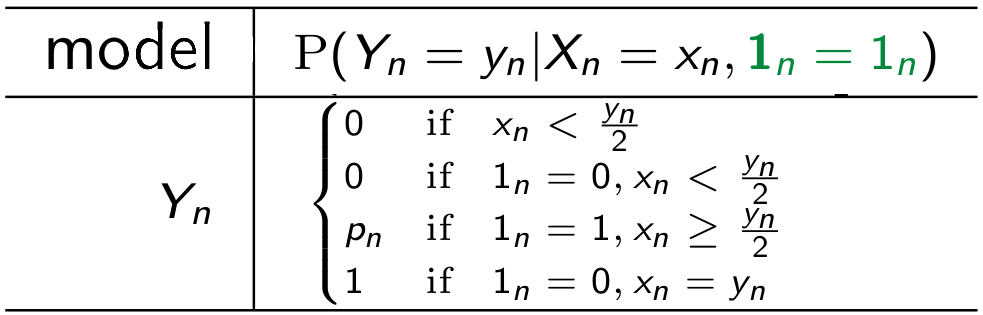
\includegraphics[height=2cm,width=5cm]{emission.png}
\end{center}
\begin{itemize}
 \item $p_n$ can be computed through the following recursive relation:
\end{itemize}
\begin{equation}
p_n = \frac{1}{n(1-\phi_1 - \phi_2)} [\phi_1 (x_n - (n-1))p_{n-1} + \phi_2 (x_n - (n-2))p_{n-2}]
\end{equation}
\end{frame}

\section{Results}
\subsection{Simulation study}
\begin{frame}{Simulation study}
\begin{itemize}
 \item In order to evaluate the model capabilities for under-reporting and over-reporting
detection and estimation two time series are simulated, one with overreporting
and another with under-reporting
 \item Although we here know which time series is over- and under-reported, the model also provides an
easy mechanism for identifying which misreporting phenomenon is present in the
data
\end{itemize}
\end{frame}

\begin{frame}{Results}
\begin{table}[ht]\small
\begin{center}
\begin{tabular}{lccccc}
\hline
& \multicolumn{5}{c}{Over-reporting}\\
& $\alpha$&$\lambda$&$\omega$&$\phi_1$&$\phi_2$\\
 \hline
true parameter & 0.3 & 3.0 & 0.7& 0.1& 0.8\\
point estimate & 0.3578 & 3.2684 & 0.5501 & 0.0771 &0.8072 \\
std. error &  0.1054 & 0.7352 & 0.1155 & 0.0297 & 0.0829 \\
\hline \hline 
& \multicolumn{5}{c}{Under-reporting}\\
& $\alpha$&$\lambda$&$\omega$&$\phi_1$&$\phi_2$\\
 \hline
true parameter & 0.5 & 3.0 & 0.7& 0.2& 0.1\\
point estimate & 0.5184 & 3.0586 &  0.7354 & 0.1952  & 0.0784 \\
std. error & 0.1554 & 0.8808 & 0.0890 & 0.0511 & 0.0339 \\
\hline 
\end{tabular}
\end{center}
\end{table}
\end{frame}

\begin{frame}{Results}
We also compared several theoretical and empirical moments for both simulated
time series, such as the mean, variance, and the first auto-correlation coefficients
\begin{itemize}
 \item For the over-reported time series, we observed a mean and variance
of 7.00 and 13.65, respectively, while the corresponding theoretical values are 6.91
and 14.31. With respect to the first auto-correlation coefficients, we observed
${\hat \rho}(1) = 0.192$, ${\hat \rho}(2) = 0.126$, and ${\hat \rho}(3) = 0.037$, while the corresponding theoretical
values are $\rho(1) = 0.2183$, $\rho(2) = 0.0655$ and $\rho(3) = 0.0196$.
\end{itemize}
\end{frame}

\begin{frame}{Results}
\begin{itemize}
 \item For the under-reported time series, the empirical mean and variance were $3.34$ and $7.52$ compared to the theoretical ones that were $3.40$ and $6.82$. The first three coefficients of the empirical auto-correlation were here ${\hat \rho}(1)=0.163$, ${\hat \rho}(2)=0.101$, and ${\hat \rho}(3)=0.073$ compared to the theoretical ones that were  $\rho(1)=0.1433$, $\rho(2)=0.0717$ and $\rho(3)=0.0358$
\end{itemize}
\end{frame}

\section{Conclusions}

\begin{frame}{Conclusions}
\begin{itemize}
 \item Several methodological approaches have been proposed recently to face underreported data based on count time series, but few can handle also overreported data
 \item The proposed model appropriately identifies whether the time series is over-reported or under-reported, and the true values of the parameters are always contained in the 90\% Wald confidence intervals
 \item Among other applications, the proposed model can be applied to analyse the impact of the Covid-19 in health services usage
\end{itemize}
\end{frame}
%\subsection{Algorithmen analysieren}
%\begin{frame}{Algorithmuseigenschaften}
%    \begin{itemize}
%        \item Zu Beginn gilt es einige Begriffe zu klären: \begin{description}[Elementaroperation]
%            \item[Prozess] Die Ausführung der Schritte eines Algorithmus
%            \item[Prozessor] Der Ausführende (Mensch, Computer, \ldots)
%            \item[Elementaroperation] Eine einzelne, eindeutige Handlung.
%        \end{description}
%    \end{itemize}
%\end{frame}

%\begin{frame}[c]{Eigenschaften für die Analyse}
%    \twosplit{%
%    \begin{block}{Korrektheit}
%        Ein Algorithmus ist korrekt, wenn er für jede (definierte) Eingabe, die korrekte Ausgabe erzeugt.
%    \end{block}
%    \begin{block}{Partielle Korrektheit}
%        Wenn der Algorithmus terminiert, ist er korrekt.
%    \end{block}
%    }{%
%    \begin{block}{Robust}
%        Ein Algorithmus ist (maximal) robust, wenn er falsche Eingabe erkennen und abfangen kann.
%    \end{block}
%    \begin{block}{Totale Korrektheit}
%        Der Algorithmus ist partiell korrekt und terminiert.
%    \end{block}
%    }
%\end{frame}

%\begin{frame}{Eigenschaften für die Analyse}
%    \begin{itemize}
%        \item Die Begriffe sind zu unterscheiden!
%        \item So können bei einem Algorithmus verschiedene Wege zum selben Ziel führen.
%        \item (Sinnfreies) Beispiel: Der Algorithmus kann jedes Element eines Arrays quadrieren. Die Reihenfolge wählt er zufällig aus!
%        \item Dieser Algorithmus \emph{determiniert}, ist aber \emph{nicht-deterministisch}!
%    \end{itemize}
%\end{frame}

%\begin{frame}{Bibliography}
    %\printbibliography
%\end{frame}

\end{document}